% !TeX spellcheck = en_GB

\documentclass[preprint,12pt]{elsarticle}
%% Use the option review to obtain double line spacing
%% \documentclass[preprint,review,12pt]{elsarticle}

\usepackage{lmodern}
\usepackage[utf8]{inputenc}
\usepackage[english]{babel}

%% Use the options 1p,twocolumn; 3p; 3p,twocolumn; 5p; or 5p,twocolumn
%% for a journal layout:
%% \documentclass[final,1p,times]{elsarticle}
%% \documentclass[final,1p,times,twocolumn]{elsarticle}
%% \documentclass[final,3p,times]{elsarticle}
%% \documentclass[final,3p,times,twocolumn]{elsarticle}
%% \documentclass[final,5p,times]{elsarticle}
%% \documentclass[final,5p,times,twocolumn]{elsarticle}

%% The graphicx package provides the includegraphics command.
\usepackage{graphicx}
\usepackage{amssymb}
\usepackage{amsmath,empheq, amsfonts}
\usepackage{subcaption}
\usepackage[section]{placeins}

\usepackage{amsthm}
\newtheorem*{remark}{Remark}

%% The amsthm package provides extended theorem environments
%% \usepackage{amsthm}

%% The lineno packages adds line numbers. Start line numbering with
%% \begin{linenumbers}, end it with \end{linenumbers}. Or switch it on
%% for the whole article with \linenumbers after \end{frontmatter}.
\usepackage{lineno}

% Pseudocode
\usepackage{algorithm2e}
\SetKw{KwBy}{by}

%% natbib.sty is loaded by default. However, natbib options can be
%% provided with \biboptions{...} command. Following options are
%% valid:

%%   round  -  round parentheses are used (default)
%%   square -  square brackets are used   [option]
%%   curly  -  curly braces are used      {option}
%%   angle  -  angle brackets are used    <option>
%%   semicolon  -  multiple citations separated by semi-colon
%%   colon  - same as semicolon, an earlier confusion
%%   comma  -  separated by comma
%%   numbers-  selects numerical citations
%%   super  -  numerical citations as superscripts
%%   sort   -  sorts multiple citations according to order in ref. list
%%   sort&compress   -  like sort, but also compresses numerical citations
%%   compress - compresses without sorting
%%
%% \biboptions{comma,round}

% \biboptions{}

\journal{Neurocomputing}

\begin{document}

\begin{frontmatter}

%% Title, authors and addresses

\title{Sparse, Robust Least Squares Support Vector Machines for the Classification of noisy datasets}

%% use the tnoteref command within \title for footnotes;
%% use the tnotetext command for the associated footnote;
%% use the fnref command within \author or \address for footnotes;
%% use the fntext command for the associated footnote;
%% use the corref command within \author for corresponding author footnotes;
%% use the cortext command for the associated footnote;
%% use the ead command for the email address,
%% and the form \ead[url] for the home page:
%%
%% \title{Title\tnoteref{label1}}
%% \tnotetext[label1]{}
%% \author{Name\corref{cor1}\fnref{label2}}
%% \ead{email address}
%% \ead[url]{home page}
%% \fntext[label2]{}
%% \cortext[cor1]{}
%% \address{Address\fnref{label3}}
%% \fntext[label3]{}


%% use optional labels to link authors explicitly to addresses:


\author[statistics]{Iwein Vranckx\corref{mycorrespondingauthor}}
\cortext[mycorrespondingauthor]{Corresponding author}
\ead[url]{wis.kuleuven.be/stat/robust}
\ead[mail]{iwein.vranckx@kuleuven.be}

\author[stadius]{Joachim Schreurs}
\author[mebios]{Bart De Ketelaere}
\author[statistics]{Mia Hubert}
\author[stadius]{Johan Suykens}
%
\address[statistics]{KU Leuven, Department of Mathematics and LStat, Celestijnenlaan 200B, BE-3001 Heverlee, Belgium}
\address[stadius]{KU Leuven, ESAT-STADIUS, Kasteelpark Arenberg 10, BE-3001 Heverlee, Belgium}
\address[mebios]{KU Leuven, Division of Mechatronics, Biostatistics and Sensors, Kasteelpark Arenberg 30, BE-3001 Heverlee, Belgium}

\begin{abstract}
(Abstract uit weighted LS-SVM, ter voorbeeld). Least squares support vector machines (LS-SVM) is an SVM version which involves
equality instead of inequality constraints and works with a least squares cost function.
In this way, the solution follows from a linear Karush–Kuhn–Tucker system instead of
a quadratic programming problem. However, sparseness is lost in the LS-SVM case and
the estimation of the support values is only optimal in the case of a Gaussian distribution
of the error variables. In this paper, we discuss a method which can overcome these two
drawbacks. We show how to obtain robust estimates for regression by applying a weighted
version of LS-SVM. We also discuss a sparse approximation procedure for weighted and
unweighted LS-SVM. It is basically a pruning method which is able to do pruning based
upon the physical meaning of the sorted support values....

The methods of this paper are illustrated for RBF kernels and demonstrate how to obtain
robust estimates with selection of an appropriate number of hidden units, in the case of
outliers or non-Gaussian error distributions with heavy tails

\end{abstract}

\begin{keyword}
	Robust support vector machines\sep Non-linear outlier detection \sep Support vector pruning \sep Sparse LS-SVM 
\end{keyword}
\end{frontmatter}

%\linenumbers

%% main text
\section{Introduction}

The least-squares support vector machines (LS-SVM) is powerful method for solving pattern recognition and regression problems~\cite{suykens2002least}. The LS-SVM maps the data to a higher dimensional space in which one constructs an optimal separating hyperplane. It has been applied to many real-world problems such as optimal control~\cite{suykens2001optimal}, financial time series prediction~\cite{van2001financial}, system identification~\cite{goethals2005identification}, electrical load forecasting~\cite{espinoza2006fixed} and many others. However the LS-SVM has two main disadvantages. It is sensitive to outliers which have large support values resulting from the solution to the linear system. The second disadvantage is that the solution lacks sparseness, which is essential for real-time prediction with big-data.

To reduce the influence of outliers, Suykens et al.~\cite{suykens2002weighted} proposed the weighted LS-SVM. By iteratively assigning small weights to outliers and retraining, the method diminishes the effect of extreme values. Another solution was proposed by Yang et. al~\cite{yang2014robust}, where a truncated loss function is used in the objective which is solved by a concave-convex procedure and the newton algorithm. A third solution is suggested by Debruyne et. al~\cite{debruyne2009robustified}, which proposes a weighted LS-SVM classification where weights are equal to spatial rank with respect to the other feature vectors in the group.

In comparison to the standard Support Vector Machines (SVM), the LS-SVM only requires solving a linear system, but it lacks sparseness in the number of solution terms. To solve this problem, Suykens et. al~\cite{suykens2000sparse} propose a method that iteratively prunes the datapoints with lowest support values and retrains. Yang et.al~\cite{yang2014sparse} propose a one-step compressive pruning strategy to reduce the number of support vectors. Fixed-size LS-SVM sparsifies the LS-SVM by selecting important point or landmark points based on the quadratic Renyi Entropy criterion~\cite{suykens2002least}. However the landmark points are fixed in advance and don't take into account information of the classification itself, which could lead to sub-optimal results. This is in contrast to the sparse LS-SVM~\cite{suykens2000sparse}, which chooses datapoints based on the impact on the classification boundary. A comparison of different pruning methods can be found in~\cite{hoegaerts2004comparison}. 

In this paper, we propose a method to solve the two problems at once.
Our mean contributions consist off:
\begin{enumerate}
	\item Kernel Concentration steps for outlier detection
	\item Soft reweighting based on Stahel-Donoho outlyingness
	\item A new Pruning strategy based on Entropy and determinantal point processes (DPP)
\end{enumerate}

Other methods that try to tackle both problems at once are found in~\cite{chen2018sparse}, where a primal formulation of the LS-SVM with a truncated loss is introduced, sparseness is obtained by the Nystr\"{o}m approximation. A second method is the weighted LS-SVM of Suykens et. al~\cite{suykens2002weighted}. \\


NOG AANPASSEN
The remainder of this paper is organized as follows. In section 2 we introduce our sparse robust least squares support vector machine. In section 3 we propose our robust outlier detection routine, followed by our support vector sparseness routine (??). The extensive simulation results of both theoretical and real, industrial datasets listed in section 4 conform the robustness, prediction time speed-up and improved classifier efficiency of our proposed method. Finally, our main findings and suggestions for further research are summarized in the conclusion, section 5. 


\section{LS-SVM for classification}
A binary classifier's goal is to learn a prediction model that assigns the correct label $y \in \{+1, -1\}$ to an unseen test sample. Restated more formally, we seek an SVM-based classifier that fits an optimal hyperplane between the two classes, where the hyperplane maximizes the distance to the closest point(s) of either class. This margin $||w||^{-1}$ maximization leads directly to a classifier with good generalisation properties, i.e: it will result in good classification performance on (unseen) test data, for example compared with density based estimators. \\

%%%%%%%%%%%%%%%%%%%%%%%%%%%%%%%%%%%%%%%%%%%%%%%%%%%%%%%%%%%%%%%%%%%%%%%%%%%%%%%%%%%%%%%%%%	
%%%%%%%%%%%%%
%%%%%%%%%%%%%	AANPASSEN AAN WEIGHTED LEAST SQUARES PRINCIPE

Given an $p$-variate trainingsset $x \in \mathbb{R}^p$ and the binary class label $y_i \in[+1,-1]$ for observation $x_i$ with index $i$, the following constrained optimization must be solved to obtain the LS-SVM representation of a support vector machine:

\begin{equation}
min \  J(w,b,e_i) = \frac{1}{2} w^T w + \frac{\gamma}{2} \sum_{i=1}^{n} e_i^2
\label{eq:costfunction}
\end{equation}
...subject to the equality constraints:
\begin{equation}
y_i[w^T \varphi(x_i) + b] = 1-e_i
\label{eq:lsconstraint}
\end{equation}

Here $w^T \varphi(x_i) + b$ is the hyperplane based decision function of the classifier with corresponding parameters $w$ and $b$, where the scalar $\gamma$ is used to control the over/under-fitting trade-off. Finally,  $\varphi(.)$ is the transformation from input space $\mathbb{R}^p$ to the kernel feature space, abbreviated as $\mathcal{H}$. \\

The specified constraint states that every given multivariate sample should be lie on the correct side of hyperplane. Stated differently, the classifier should predict the class label of each sample correctly, where each observation $x_i$ has an corresponding error $e_i$ due to the constraint equality sign. This, in turn, implies that a LS-SVM loses its support vector sparseness compared to ordinary SVM's. \\

This constrained optimization problem is solved by the optimality conditions of its Lagrangian $\alpha$ as follows:
\begin{equation}
L(w,b,e;\alpha) = J(w,b,e) - \sum_{i=1}^{n} \alpha_i(y_i [ w^T \varphi(x_i) + b]-1 + e_i)
\label{eq:lagrangian}
\end{equation}
%Here, $\alpha_i$ is the Lagrange multiplier whose value can be either positive or negative, which is also different from the standard SVM proposed by Vapnik. 
As a direct consequence of the equality sign in the given constraint the specified Lagrangian is now solvable trough a linear system of equations:
\begin{align}
\frac{\partial L}{\partial w} &= 0 \rightarrow w = \sum_{i=1}^{n} \alpha_i y_i \varphi(x_i) \\
\frac{\partial L}{\partial b} &= 0 \rightarrow \alpha^T y = 0 \\
\frac{\partial L}{\partial e} &= 0 \rightarrow \alpha = \gamma e \\
\frac{\partial L}{\partial \alpha_i} &= 0 \rightarrow y_i [w^T \varphi(x_i) + b ] = 1 - e_i 	
\end{align}
Combining the first and last equation and defining $\Omega{(i,j)}$ for two observations with index $i$ and $j$ as:
\begin{align}
\Omega{(i,j)} &= y_i y_j \varphi(x_i)^T \varphi(x_j) \\
&= y_i y_j K(x_i, x_j)
\end{align}
Yields the following set of linear equations, where the kernel matrix $K$ transforms observations to the high dimensional kernel feature space $\mathcal{H}$.

\begin{equation}
	\begin{bmatrix}
		0 & y^T \\
		y & \Omega + \gamma^{-1} \mathbf{I}
		\end{bmatrix}	
		\begin{bmatrix}
		b \\
		\alpha
		\end{bmatrix}
		=
		\begin{bmatrix}
		0 \\
		\mathbf{1}
	\end{bmatrix}	
\end{equation}
The least squares solution of the aforementioned system of equations is then used to  obtain the Lagrange coefficients $\alpha$ and offset $b$, where the decision function used for test set prediction is defined as:
\begin{equation}
	\hat{y}(x) = \sum_{1}^{n} \alpha_i y_i K(x, x_j) + b	
	\label{eq:classification}
\end{equation}
Or, written in a more convenient matrix notation, short-writing $\beta_i= (\alpha_i \  y_i)^T$
\begin{equation}
	\hat{y}(x) = \mathbf{\beta} K + b \mathbf{1}
	\label{eq:prediction}
\end{equation}
$\hat{y}_i$ is the predicted output of the ith training data point. Note that $\alpha$ satisfies the linear constraint $\sum_{i=1}^{n} \alpha_i  e_i = 1$, and that the derivation for least squares support vector regression follows the same reasoning (DOES IT??) %\cite{Choi2009}.

\newpage

\section{Proposed method}
%We first start by laying out the main methodology of our proposed robust, sparse SVM algorithm. \\
%Korte paragraaf met schema of uitleg van het algoritme:
%\begin{enumerate}
%	\item Outlier detection by kernel Csteps: [WAT IS DE IMPACT VAN OUTLIERS EN WAAROM??]
%	\item solve system of equations
%	\item Imposing sparseness
%	\item Samping strategy: 
%	\begin{enumerate}
%		\item Entropy (?)
%		\item DPP
%	\end{enumerate}
%	\item information transfer.
%\end{enumerate} 
%
%\newpage
\subsection{Concentration steps in kernel feature space}

Having introduced the LS-SVM model, our attention first goes to the detection of outliers in the dataset. Modern multivariate robust statistical methods are frequently based on the Minimum Covariance Determinant (MCD) method, first introduced in  (Rousseeuw, 1984, 1985). This Mahalanobis distance based estimator can withstand a substantial amount of trainingset contamination (up to 50\%), and is nowadays (also) employed as the a refinement step of an initial estimator. This two-step mechanism inherits the robustness of the MCD, but offers an improved statistical efficiency [see e.g. REF: DetS, detMM]. Deterministic variants and well know PCA-based applications are described in [detMCD, RobPCA] respectively. \\

Given a trainingset $X$ of $n$ observations in $p$ dimensions, the MCD-objective is to find the $h$ observations whose sample covariance matrix has the lowest possible determinant, where the amount of regular observations $h < n$ is specified before the algorithm starts. The MCD-estimate of location $c_h$ is then the average of these $h$ points (the $h$-subset), whereas the scatter estimate is a multiple of their covariance matrix $\hat{\Sigma}_{h}$. 

In order to find the MCD-estimate, the FastMCD-algorithm (Rousseeuw and Van Driessen, 1999) uses so-called concentration steps (C-steps). These iterative algorithm steps result in a decreasing covariance matrix determinant: a goodness-of-fit metric [BLABLABLA]. Based on its robustness properties, simplicity and proven convergence, we propose to modify the algorithm in way that it can work in kernel feature space, where it is used to for the detection of \textit{non-linear} outliers: a noteworthy difference compared to off-the-shelve robust statistical algorithms as normality is always assumed. \\

To enable the C-steps methodology $\mathcal{H}$, we integrate the mapping function $\phi(.)$ in the required algorithm formula's: 
\begin{equation}
	\label{eq:center}
	c_h = \frac{1}{h} \sum_{i=1}^{h}\phi(x_i)
\end{equation}
Likewise, the Mahalanobis distance in $\mathcal{H}$ is defined as:
\begin{equation}
	\label{eq:smd}
	||\phi(x) - c_h||^2_{\Sigma_h} = (\phi(x) - c_h) \Sigma^{-1}_h (\phi(x) - c_h)
\end{equation}
Where the biased covariance matrix of the $h$-subset is calculated as:
\begin{equation}
	\Sigma_h = \frac{1}{h} \sum_{i=1}^{h} (\phi(x_i) - c_h) (\phi(x_i) - c_h)^T
	\label{eq:sigma}
\end{equation}
As we do not explicit know the mapping function $\phi(.)$, equation \ref{eq:smd} cannot be calculated, a problem circumvented by the singular value decomposition of the covariance matrix:
\begin{equation}
	\Sigma_h = V^T D V
\end{equation}
Where $V$ is the matrix of eigenvectors $v^k$ and $D$ resembles the diagonal matrix of eigenvalues $\lambda^k$ for $k=1,2, \dots, h$. The relation between eigenvalues and eigenvectors follows the identity:
\begin{equation}
	\label{eq:eigenrelation}
	\Sigma_h v^k = \lambda^k v^k
\end{equation} 
From the definition of equation \ref{eq:sigma}, it can be seen that each eigenvector is a linear combination of the observations $\phi(x_i)$ in kernel feature space:
\begin{equation}
v^k = \sum_{1}^{n} \alpha_i^k ( \phi(x_i) - c_n) 
\end{equation}
If we substitute the above in equation \ref{eq:eigenrelation}, it follows that:
\begin{equation}
	n \lambda^k \alpha^k = \tilde{K} \alpha^k
\end{equation}
Here, $\tilde{K}$ denotes the symmetric kernel matrix of $h$ rows, centred in $\mathcal{H}$. The weights $\alpha$ are determined by solving the eigendecomposition problem. \\
By refactoring $\Sigma^{-1}$ as $V^T D^{-1/2} D^{-1/2} V$ and exploiting reductant operations in the Mahalanobis distance formula, [REF: NADER] proofs that equation \ref{eq:smd} can be calculated in $\mathcal{H}$ as:
\begin{equation}
	||\phi(x) - c_n||^2_{\Sigma} = \sum_{k=1}^{n} (\lambda^k)^{-1} \big( \sum_{k=1}^{n} \alpha^k \tilde{k}(x_i, x) \big)^2
\end{equation}	

Finally, the centred kernel matrix of the $h$-subset $\tilde{K}_h$ is calculated as [REF: cite Nonlinear Component Analysis as a Kernel Eigenvalue Problem]:
$ \tilde{K}^{(hh)} \in \mathbb{R}^{h \times h}$ and $1_h \in \mathbb{R}^{h}$ with all entries set to $1/h$
\begin{align}
\label{eq:centerKh}
	\tilde{K}_{ij}^{(hh)} &= \Big(\phi(x_i) - \frac{1}{h}\sum_{m=1}^h\phi(x_m)\Big) \cdot \Big(\phi(x_j) - \frac{1}{h}\sum_{n=1}^h\phi(x_n)\Big) \\
						  &= K_{ij}^{(hh)} - \frac{1}{h}\sum_{m=1}^h K_{mj} - \frac{1}{h}\sum_{n=1}^h K_{in} + \frac{1}{h^2}\sum_{m=1}^h\sum_{n=1}^h K_{mn} \\
						  &= \Big(K^{(hh)} - 1_h K^{(hh)} - K^{(hh)}1_h + 1_h K^{(hh)}1_h\Big)_{ij}
\end{align}
Where the centring of the kernel matrix of $n$ observations, given the $h$-subset follows the similar derivation. Define the kernel matrix $ \tilde{K}^{(h)} \in \mathbb{R}^{n \times h}$ and $1_h \in \mathbb{R}^{h \times n}$ with all entries set to $1/h$

\begin{align}
	\tilde{K}^{(h)} &= K^{(h)} - 1_h^T K^{(hh)} - K^{(h)}1_h + 1_h^T K^{(hh)}1_h
\end{align}
	

\subsection{The proposed C-step in kernel feature space}

We first standardize each dataset observation by $z_i = (x_i - \hat{\mu}_{mcd}) / \hat{\sigma}_{mcd}$ where $\hat{\mu}_{mcd}$ and $\hat{\sigma}_{mcd}$ are the univariate location and scale estimations of the univariate MCD[REF]. This reduces the impact of different feature scales. Next, the standardized dataset is split in two subsets according to its class label $y \in \{+1, -1\}$ and our proposed  procedure is applied (per subset) to derive at an outlier free support vector candidate set. 

\begin{itemize}
	\item [Step 1] Calculate the spatial median in $\mathcal{H}$, as introduced in [MICHIEL]. The spatial median can be written as a linear combination of the feature vectors. Denote $\gamma = (\gamma_1, \dots, \gamma_n)^T$ the vector of coefficients, where it is know that $\sum_{i=1}^{n} \phi(x_i) \gamma_i$ equals the spatial median in feature space. Initialise $\gamma = (1/n, 1/n, \dots)$ and recursively compute the normalized coefficients $\gamma = w / \sum_{i=1}^{n}w_i$, where $w_i$ for the observation with index $i$ is calculated as:
	\begin{equation}
		w_i = \frac{1}{\sqrt{ K_{i,i} - 2 \gamma^T K_{., i} + \gamma^T K \gamma}}
	\end{equation}
	Ten iterations are used to obtain a good approximation.	
	\item [Step 2] Calculate the Euclidean distance for each observation to the spatial median:
	\begin{align}
	d_i &= || \phi(x_i) - \sum_{j=1}^N \gamma_j \phi(x_j)||^2 \\
	&= || \phi(x_i)||^2 + || \sum_{j=1}^N \gamma_j \phi(x_j)||^2 - 2 <\phi(x_i),\sum_{j=1}^N \gamma_j \phi(x_j)> \\
	&= K(x_i,x_i) + \sum_{j=1}^N \sum_{k=1}^N \gamma_j \gamma_k K(x_j,x_k) - 2 \sum_{j=1}^N\gamma_j K(x_i,x_j)
	\end{align}
	\item [Step 3] 	Sort these distances is ascending order. Define the initial $h$-subset of $h_{init}$ observations with the lowest distance.	

	\item [Step 4] Apply kernel C-step for a fixed amount of iterations as follows:

	\begin{enumerate}
		\item Calculate the kernel matrix for the given $h$-subset of observations and kernel.
		\item Center $K$ in $\mathcal{H}$ by equation \ref{eq:centerKh}, obtaining $\tilde{K}_h$
		\item Perform the singular value decomposition on $\tilde{K}_h$ to obtain the eigenvectors $\alpha$ and eigenvalue vector $L_d$ (equation [..]).
		\item Normalize each eigenvector $\alpha_i$ by its corresponding eigenvalue, equation [...]
		\item Calculate the kernel matrix for the given $h$-subset of observations in $n$ features.
		\item Center the kernel matrix by equation [REF..] and obtain the malalanobis distances with equation [REF].
		\item Sort these Mahalanobis distances in ascending order and redefine the $h$-subset as the $h$ observations with smallest distance.
		\item If the new $h$-subset is equal to the previous one, exit the C-step loop.
	\end{enumerate}

%	\begin{enumerate}	
%		\item For each observation $x$, calculate the corresponding Mahalanobis distance, defined as:
%		\begin{equation}
%		||x - c_h||^2_{\Sigma_h} = (x - c_h) \Sigma^{-1}_h (x - c_h)
%		\end{equation}	
%		\item Sort the Mahalanobis distances in ascending order. Redefine the $h$-subset with the $h$ observations with lowest distance. 
%		\item Obtain a new estimation of location and scatter:
%		\begin{align}
%		c_h &= \frac{1}{h} \sum_{i=1}^{h}x_i \\
%		\Sigma_h &= \frac{1}{h} \sum_{i=1}^{h} (\phi(x_i) - c_h) (\phi(x_i) - c_h)^T 
%		\end{align}
%		
%		\item Re-iterate until a specified number of steps or until no convergence is obtained:
%		\begin{equation}
%		\det(\hat{\Sigma}_h(t))=\det(\hat{\Sigma}_h(t-1))
%		\end{equation}
%	\end{enumerate}

	\item [Step 5] If the $h$-subset size is lower then $h_{end}$, increase the $h$-subset size by (say) 5\% and go back to step 4. 
	\item [Step 6] Determine the final support vector candidate mask. Assign a binary weight to each observation $i$:
	\begin{equation}
	w_i =
	\begin{cases}
	1, & \text{if}\ rd^2(i) \leq max(\chi^2_{0.975, p}, rd^2(h-subset)) \\
	0, & \text{otherwise}
	\end{cases}
	\end{equation}
\end{itemize}
The different steps of this algorithm are shown in figure [REF], where it can be seen that [WAT]. The final outcome, weights for each observation, are kept in memory to ...; Next, we solve the system of equations

\begin{enumerate}
	\item Group the weights
	\item item SOLVE THE SYSTEM OF EQUATIONS CFR EQUATION 
\end{enumerate}
This yields $\alpha$, the supprt vector candidate list,  ... and ...

\begin{figure}[!htb]
	\centering
	\begin{subfigure}[b]{0.40\linewidth}
		\centering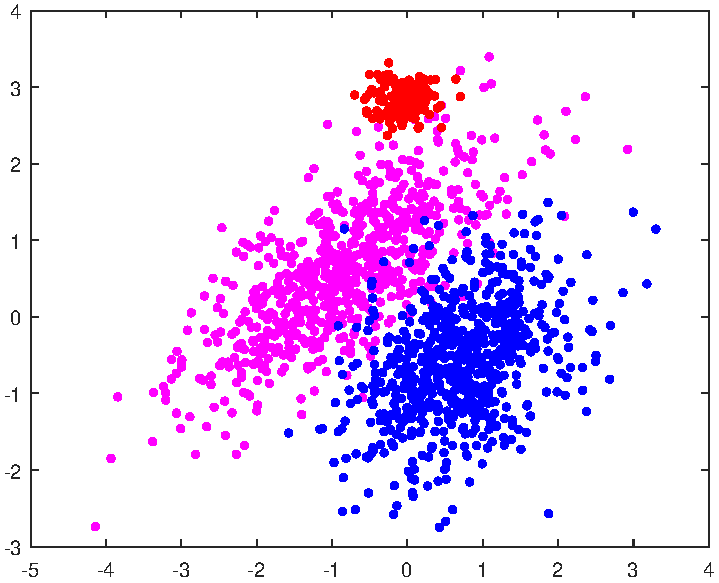
\includegraphics[width=1\linewidth]{figures/kcstep/nddatamodel.pdf}
		\caption{\label{fig:dmodel}} 
	\end{subfigure}
	\begin{subfigure}[b]{0.40\linewidth}
		\centering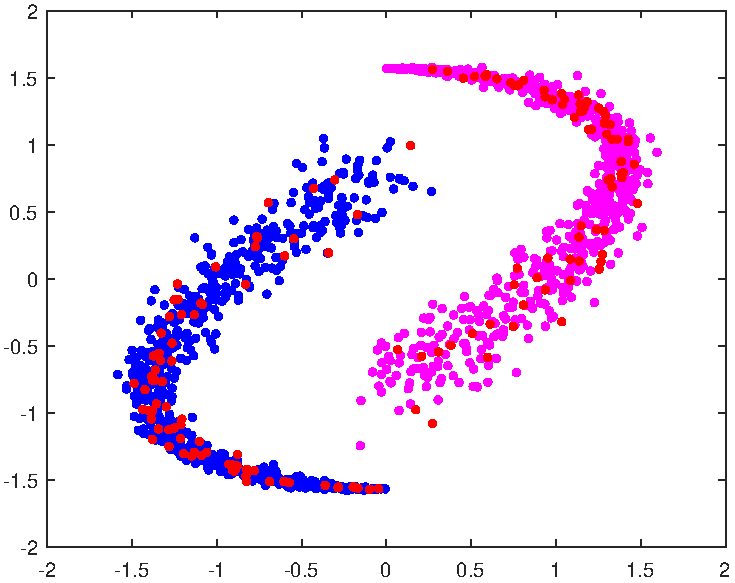
\includegraphics[width=1\linewidth]{figures/kcstep/yydatamodel.pdf}
		\caption{\label{fig:dmodel}} 
	\end{subfigure} \\

	\begin{subfigure}[b]{0.40\linewidth}
		\centering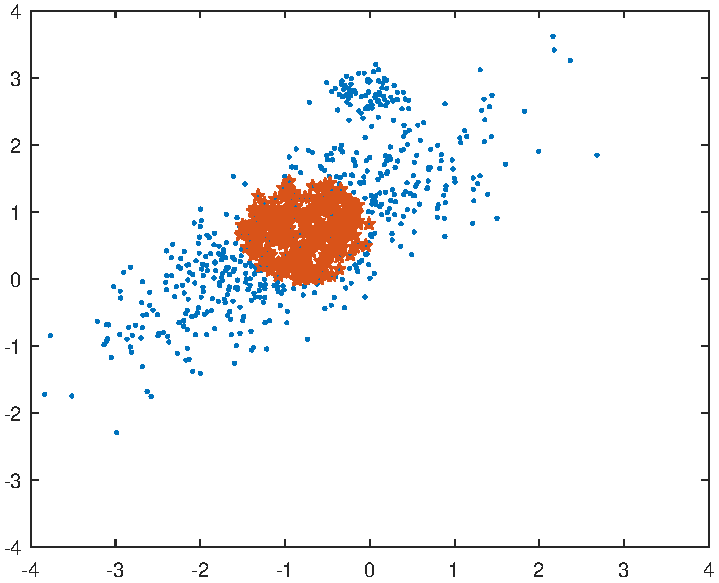
\includegraphics[width=1\linewidth]{figures/kcstep/c1input.pdf}
		\caption{\label{fig:spatialmedc1}}
	\end{subfigure}
	\begin{subfigure}[b]{0.40\linewidth}
		\centering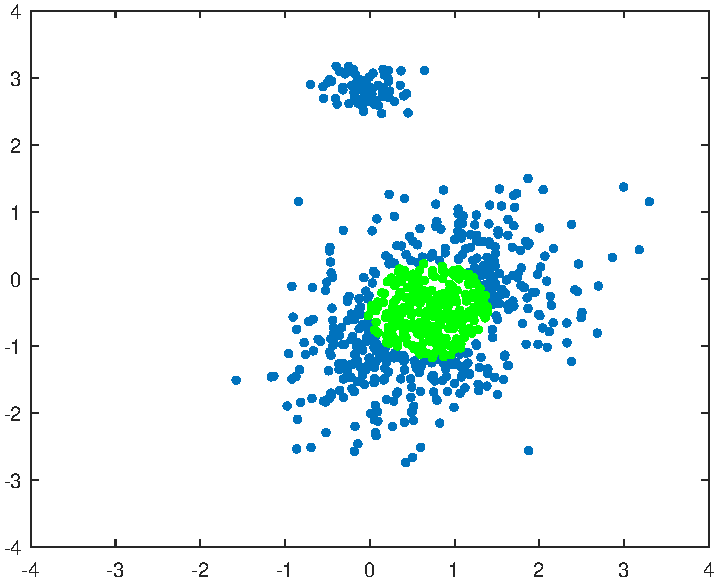
\includegraphics[width=1\linewidth]{figures/kcstep/c2input.pdf}
		\caption{\label{fig:spatialmedc2}}
	\end{subfigure} \\

	\begin{subfigure}[b]{0.40\linewidth}
		\centering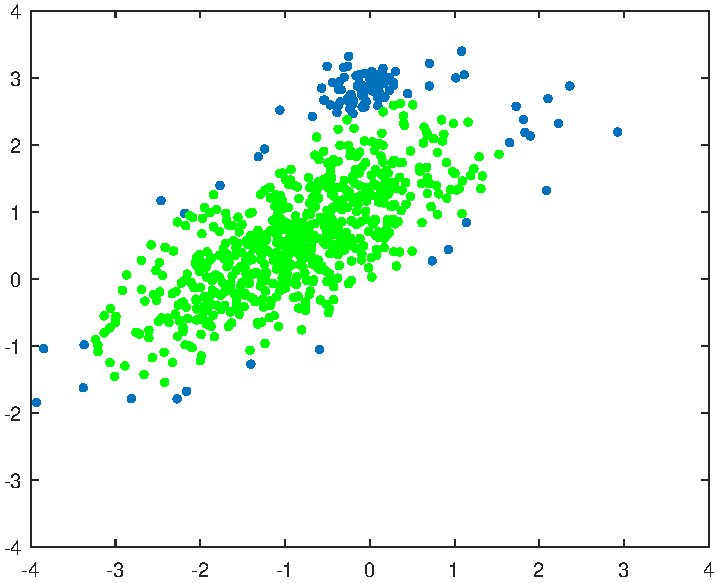
\includegraphics[width=1\linewidth]{figures/kcstep/c1output.pdf}
		\caption{\label{fig:kcstepc1}}
	\end{subfigure}
	\begin{subfigure}[b]{0.40\linewidth}
		\centering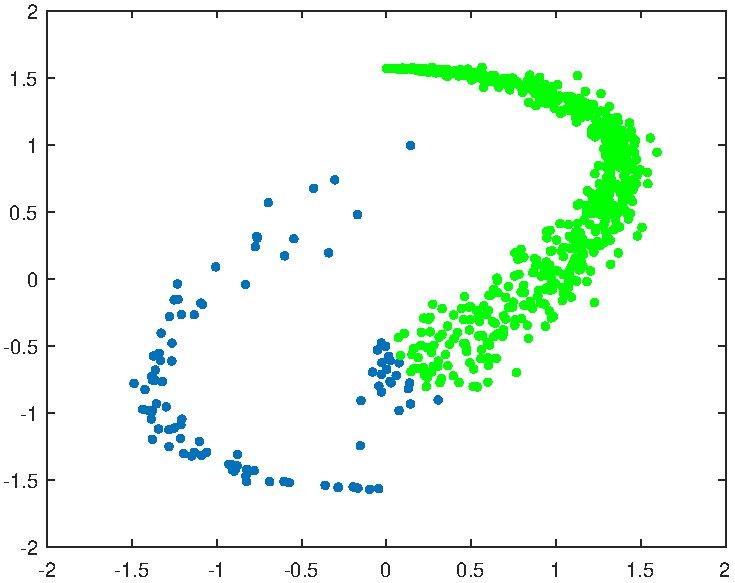
\includegraphics[width=1\linewidth]{figures/kcstep/c2output.pdf}
		\caption{\label{fig:kcstepc2}}
	\end{subfigure}

	\caption{
		Figure \subref {fig:dmodel} depicts a normal distributed, binary classification problem. Both classes (blue, green) contain $10\%$ outliers from the same material group, shown in red. After splitting the dataset by their class labels [STEP2?], the $h_ {init} $ closest points from the spatial median are used as initial subsets for the C-step algorithm [STEP3?], depicted in green for both classes (figure b, c). After iterative kernel C-steps we obtain the re-weighted results  [STAP5?], shown in figures d and e. Support vectors are then determined from the detected regular observation list by a landmark selection algorithm (section [REF]).}
\end{figure}
 


\newpage
\FloatBarrier

\section{Imposing sparseness}

\subsection{Selection of the best support vectors}

Having established the data model and optimized classification accuracy for contaminated datasets, let us return to the problem at hand: the development of a pruning strategy. This implies that prediction formula should be partitioned in a \textit{relevant} (the support vectors or landmark points, found by the pruning algorithm) - and \textit{irrelevant} part.  An overview of existing pruning methods can be found in Hoegaerts et. al \cite{hoegaerts2004comparison}. A first approach was suggest by Suykens et. al \cite{suykens2000sparse}, where  sparseness is imposed by pruning support values from the sorted support value spectrum resulting from the solution to the linear system.  The motivation comes from the fact that LS-SVM support values are proportional to the errors at datapoints. Thus omitting the points that contribute least to the training error. An example of the support value spectrum can be seen on Figure \ref{fig:BadAlpha}. The values with a high $|\alpha_k|$ reside close to the decision boundary and are thus important to classify correctly. 

However blindly taking the points with largest support value spectrum could lead to sub-optimal results. Firstly, when outliers are present, you want to be certain that these are not chosen. Secondly, points are chosen independently towards each other. This results in clumping of landmarks. The first problem is addressed by running a kernelized minimum covariance determinant, which detects and omits potential outliers. 

The second problem is solved by introducing a "region of interest" (ROI) for each class $Y = [+1,-1]$, which consist of the points with the $\beta$ percentage highest value of $Y \alpha_iy_i$, where $\alpha_i$ and $y_i$ are the support value and class label of training point $x_i$. In contrast to the proposed pruning strategy by Suykens et. al~\cite{suykens2000sparse}, the sign of alphas is taken in consideration when determining the ROI. Potential landmark points are now points with large importance and that predict the right class. This is easily seen from the prediction equation \eqref{eq:prediction}, where the contribution of a training point in the prediction a test point $z$ towards class Y is proportional to $Y \alpha_iy_i$. 

The ROI represents a subset with points important for the decision boundary. Using a sampling algorithm that promotes diversity, $h$ landmark points are selected to represent the ROI such that no clumping is possible.


\begin{figure}[h]
	\centering
	\begin{subfigure}[b]{0.3\textwidth}
		\label{fig:BadAlpha}
		\caption{Example bad Alpha spectrum}
	\end{subfigure}
	\begin{subfigure}[b]{0.3\textwidth}
		\label{fig:GoodPruning}
		\caption{Example good SV selection}
	\end{subfigure}
\end{figure}

\subsubsection{Entropy}
Selection of the landmark points is based on quadratic Renyi entropy~\cite{girolami2002orthogonal} and the fixed size LS-SVM~\cite{suykens2002least}. The landmarks points are chosen to maximize the quadratic Renyi Entropy:
\begin{equation}
H_R = -\mathrm{log}\int p(x)^2 dx.
\end{equation}
The quadratic Renyi Entropy is approximated by the following equation\cite{girolami2002orthogonal}:
\begin{equation}
\int \hat{p}(x)^2dx = \frac{1}{N^2} 1_v^\mathrm{T}\Omega 1_v,
\end{equation}
where $1_v = [1;1;...;1]$ and a normalized kernel is assumed with respect to density estimation. In the fixed-size LS-SVM approach, one chooses a fixed working set of size $M$ which is initialized randomly. Afterwards, random points are swapped in and out. If the entropy increases, the swapped point is accepted, otherwise the original subset is kept. This process continues until the change in entropy is small or a fixed number of iterations is reached. 

In contrast to the original fixed-size LS-SVM formulation, which is used to find a representative subset for the Nystr\"{o}m approximation \cite{suykens2002least}. We propose to first determine to region of interest, which includes the points that have the highest contribution to the robust LS-SVM model. On this reduced dataset, the fixed-size LS-SVM algorithm is used to select the $h$ landmark points. This ensures that the ROI is well approximated and there is no clumping effect present. The improved sv selection for the toy-problem is visible on Figure \ref{fig:GoodPruning}.


\begin{remark}
	It is important to first omit outliers, before continuing with the entropy procedure. Large contributions to the entropy will come from elements that have little or no structure~\cite{girolami2002orthogonal}.
\end{remark}

Given an outlier free $h$-subset of candidate support vectors, the entropy based selection algorithm works as follows[REF]:
\begin{enumerate}
	\item for iteration = 1:10*size(x,1)
	\item formule 1, see equation 38 above
	\item formule 2, see equation 39 above
	\item formule ..., see [REF]
\end{enumerate}

----TODO-----
MORE EXPLANATIONS DPP


\subsubsection{Determinantal point process}
Selection of landmark points is based on determinantal point processes (DPPs)~\cite{kulesza2012determinantal}. DPPs are particularly interesting for set selection problems where diversity is preferred. A point process $\mathcal{P}$ on a ground set $\mathcal{Y} = {1,2,...,N}$ is a probability measure over point patterns of $\mathcal{C}$ , which are finite subsets of $\mathcal{Y}$. When $\mathcal{C}$ is a random subset, drawn according to the DPP $\mathcal{P}$, we have:
\begin{equation}
\label{eq:origDPP}
	\mathcal{P}(C \subseteq \mathcal{Y}) = \mathrm{det}(K_{\mathcal{C}}),
\end{equation}
where $K \preceq I$ is a positive symmetric semidefinite matrix with all eigenvalues smaller then or equal to 1, containing the index elements of $\mathcal{Y}$. $K_{\mathcal{C}} = [K_{i,j}]_{i,j \in \mathcal{C}}$ contains the selected rows and columns of $K$ and $\mathrm{det}(K_{\emptyset}) = 1$. From equation \eqref{eq:origDPP} follows:
\begin{align}
	\mathcal{P}(i \in \mathcal{Y}) &= K_{i,i} \\
	\mathcal{P}(i,j \in \mathcal{Y}) &= K_{i,i}K_{j,j} - K_{i,j}K_{j,i}\\
	\label{eq:KDPP}
	&= \mathcal{P}(i \in \mathcal{Y})\mathcal{P}(j \in \mathcal{Y}) - K_{i,j}^2.
\end{align}
The diagonal elements of the kernel matrix give the marginal probability of inclusion for individual elements of $\mathcal{Y}$, whereas the off-diagonal elements determine the (anti-)correlation between pairs of elements. Thus for large values of $K_{i,j}$, or a high similarity, points are unlikely the appear together. 

In our case, we would like to build a DPP based on the kernel matrix $K$, which is done using L-ensembles~\cite{borodin2009determinantal}. The probability of observing a subset $C \subseteq \mathcal{Y}$ is now equal to:
\begin{equation}
	\mathrm{Pr}(\mathcal{C}) = \frac{\mathrm{det}(K_{\mathcal{C}})}{\mathrm{det}(K + I)},
\end{equation}
where $I$ is the identity matrix, and $K$ a positive semidefinite matrix  indexed by the elements of $\mathcal{Y}$. In contrast to equation \eqref{eq:origDPP}, $K$ only has to be positive semidefinite, while the eigenvalues previously where bounded above. When conditioning on a fixed cardinality $k = |\mathcal{C}|$, one gets the k-DPP~\cite{kulesza2011k}.

The landmark selection algorithm consists of the following steps:
We propose to first determine to region of interest, which includes the points that have the highest contribution to the robust LS-SVM model. On this reduced dataset, a $k$-DPP~\cite{kulesza2011k}, where $k = h$, is used to sample the $h$ landmark points. This ensures that the ROI is well approximated and there is no clumping effect present. The improved sv selection for the toy-problem is visible on Figure \ref{fig:GoodPruning}.

\begin{remark}
It is important to first omit outliers, before continuing with the DPP sampling. In order to promote diversity, points that have a high similarity have a low chance of being sampled together (see equation \eqref{eq:KDPP}). Consequently outliers, that have a low similarity to any other point in the dataset, have a high chance of being sampled.
\end{remark}

Given an outlier free $h$-subset of candidate support vectors, the entropy based selection algorithm works as follows[REF]:
\begin{enumerate}
	\item for iteration = 1:10*size(x,1)
	\item formule 1, see equation 38 above
	\item formule 2, see equation 39 above
	\item formule ..., see [REF]
\end{enumerate}

\newpage
\subsection{Information transfer}
 The information contained in the prune candidates can then be transferred to the support vectors - an idea originally introduced in [???]. Starting from equation \ref{eq:prediction} with the appropriate matrix dimensions:
\begin{equation}
\hat{y}_{(1,n_2) } = \mathbf{\beta}_{(1,n_1)} K_{(n_1, n_2)} + b_{(1,1)} \ \mathbf{1}_{(1, n2)} 
\end{equation}
Introducing sparse matrices, we could partition this expression in a (non) support vector part, denoted by the subscript $S$ and $N$ respectively.
\begin{equation}
\hat{y}_{(1,n_2) } = \mathbf{\beta}_{S(1,n_1)} K_{S(n_1, n_2)} + \mathbf{\beta}_{N(1,n_1)} K_{N(n_1, n_2)} + b_{(1,1)} \ \mathbf{1}_{(1, n2)}
\end{equation}
Next, one transfers the information of $\mathbf{\beta}_{N} K_{N}$ using the update $\Delta\beta$: 
\begin{align}
\Delta \beta K_S &= \beta_N K_N  \\
\Delta \beta &= K^\dagger_S  \beta_N K_N
\end{align}
We now have obtained an explicit expression for the update of our Lagrange multipliers. 
\begin{align}
\hat{\beta}_S &= \beta_S + \Delta\beta
\end{align}
If we omit all zero rows in the matrices above we obtain a compressed matrix of size $m_1$ rows in $n_2$ dimensions. Here, $m_1$ equals the (a priori, before the training stage) defined number of support vectors. The classier prediction equation finally boils down to:
\begin{equation}
\hat{y}_{(1,n_2) } = \mathbf{\beta}_{(1,m)} K_{(m, n_2)} + b_{(1,1)} \ \mathbf{1}_{(1, n2)} 
\end{equation}
Which is implemented using equation \ref{eq:gpuprediction} given the knowledge that $n_1 = m$ - the number of a priori defined support vectors. \\

\paragraph{Algorithm 3--- summary selection of landmark points} 
\hfill \\\\
The following procedure is applied on the robust trained LS-SVM and outlierfree dataset:


%\begin{algorithm}[H]
%\KwData{$\beta \in [0,1]$, $h \in [1,N]$, $l_1,l_2 \in [1,N]$}
%$\alpha_i$, $x_i$ where $i = 1,..,h$ \gets Run algorithm 1 \\
%\For{every class $Y \in [-1 \enskip 1]$}{
%	ROI \gets largest $\beta N$ indices of $Y \alpha_v y_v$ where $v \in Y$ \\
%	idS \gets k-DPP(ROI,$l_Y$) 
%}
%Put information transfer here \\
%\Return{idS,$\alpha_S$}
%\caption{Landmark Selection}\label{Algo:LandmarkSelection}
%\end{algorithm}

\section{Experiments} 
\subsection{Simulation results} 

\subsubsection{Linear example}

Two Gaussians close, the reverse labels behind at large distance. See Robustified LS-SVM~\cite{debruyne2009robustified}

\subsubsection{Non-Linear example}

Yin-Yang, Two spiral dataset or Cross Dataset~\cite{yang2014robust}

\subsubsection{UCI}

Robust: Banana, Celveland heart, Glass, Heartstatlog, liver disorder, monk PIMA, ripley, Transfusion, Vehicle~\cite{yang2014robust}

Robust + sparse: Splice, Pendigits (choose two digits 3 vs 4), Satimage (1 vs 6), USPS (1 vs 2), Mushrooms, Protein (1 vs 2).\cite{chen2018sparse}
Outliers = 30 \% samples that where far away from decision hyperplane, then randomly sample 1/3 of them and flip labels. datasets are in https://www.csie.ntu.edu.tw/~cjlin/libsvmtools/datasets/ 

Robust: Wine dataset + Linear, Glass, Biscuit Dough, Alon colon cancer, Hepatocellular carcinoma dataset~\cite{debruyne2009robustified}. However mostly linear

\subsection{Industrial data results} 

\section{Conclusions and future work}

\section*{Acknowledgements}

We thank Johan Speybrouck for providing us the industrial datasets and Tim Wynants for his feedback throughout this project. We also acknowledge the financial support of the VLAIO, grant HBC.2016.0208, for making this industrial research possible.

%% The Appendices part is started with the command \appendix;
%% appendix sections are then done as normal sections
%% \appendix

%% \section{}
%% \label{}

%% References
%%
%% Following citation commands can be used in the body text:
%% Usage of \cite is as follows:
%%   \cite{key}          ==>>  [#]
%%   \cite[chap. 2]{key} ==>>  [#, chap. 2]
%%   \citet{key}         ==>>  Author [#]

%% References with bibTeX database:

%\bibliographystyle{model1-num-names}
\bibliographystyle{plain}
\bibliography{sample}

%% Authors are advised to submit their bibtex database files. They are
%% requested to list a bibtex style file in the manuscript if they do
%% not want to use model1-num-names.bst.

%% References without bibTeX database:

%\begin{thebibliography}{00}
%
%%% \bibitem must have the following form:
%%%   \bibitem{key}...
%%%
%
%
%\end{thebibliography}


\end{document}

%%
%% End of file `elsarticle-template-1-num.tex'.